
\section{Background}
\label{sec:background}

The current system of course selection, Webtree, was designed to allow
students to customize their course selections to deal with various
contingencies. For example, a student might want a different second
course option depending on whether or not he or she successfulling
recieved his or her first option. Webtree consists of three binary trees (depth
of $3$), which are traversed according to an elaborate
algorithm. Students' fourth class is ranked in order $1-4$, and is
selected according to availability in that order. For a visual
represention of Webtree, as well a chance to imagine the confusion that
many students feel when filling it out, see Figure~\ref{fig:webtr}.

\begin{figure}[htb]
  \centering  % centers the image in the column
  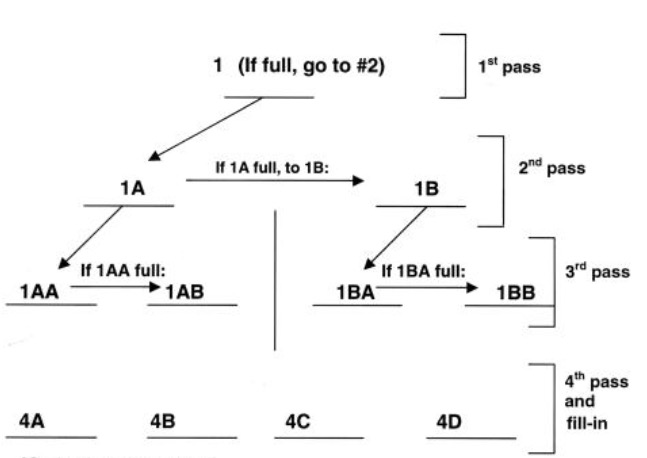
\includegraphics[width=0.37\textwidth]{figs/webtree.jpg}
  % *Every* figure should have a descriptive caption.
  \caption{The complicated nature of Davidson College's Webtree. Image
    courtesy of Davidson College Registrar.}
  \label{fig:webtr}
\end{figure}

Describe any background information that the reader would need to know
to understand your work. You do not have to explain algorithms or
ideas that we have seen in class. Rather, use this section to describe
techniques that you found elsewhere in the course of your research,
that you have decided to bring to bear on the problem at hand. Don't
go overboard here --- if what you're doing is quite detailed, it's
often more helpful to give a sketch of the big ideas of the approaches
that you will be using. You can then say something like ``the reader
is referred to X for a more in-depth description of...'', and include
a citation.\\

Alternately, you may have designed a novel approach for the problem
--- your own algorithm or heuristic, say. A description of these would
also be placed in this section (use subsections to better organize the
content in this case).




